\documentclass[11pt]{article}
\usepackage[utf8]{inputenc}

%%% PAGE DIMENSIONS
\usepackage{geometry}
\geometry{a4paper}

\usepackage{graphicx}

%%% PACKAGES
\usepackage{booktabs}
\usepackage{paralist}
\usepackage{verbatim}
\usepackage{subfig}
\usepackage{chngcntr}
\usepackage{tikz}
\usepackage[colorlinks = true,
            linkcolor = black,
            urlcolor  = blue,
            citecolor = blue,
            anchorcolor = blue]{hyperref}
\usepackage[spanish]{cleveref}
\usepackage{placeins}
\usepackage{float}
\usepackage{listings}

%%% HEADERS & FOOTERS
\usepackage{fancyhdr}
\pagestyle{fancy}
\renewcommand{\headrulewidth}{0pt}
\lhead{}\chead{}\rhead{}
\lfoot{}\cfoot{\thepage}\rfoot{}

%%% SECTION TITLE APPEARANCE
\usepackage{sectsty}
\allsectionsfont{\sffamily\mdseries\upshape}

%%% ToC (table of contents) APPEARANCE
\usepackage[nottoc,notlof,notlot]{tocbibind} % Put the bibliography in the ToC
\usepackage[titles,subfigure]{tocloft} % Alter the style of the Table of Contents
\renewcommand{\cftsecfont}{\rmfamily\mdseries\upshape}
\renewcommand{\cftsecpagefont}{\rmfamily\mdseries\upshape} % No bold!


\graphicspath{ {images/} }

\counterwithin*{figure}{section}
\counterwithin*{figure}{subsection}
\counterwithin*{figure}{subsubsection}

\counterwithin*{table}{section}
\counterwithin*{table}{subsection}
\counterwithin*{table}{subsubsection}

\addtolength{\cftfignumwidth}{2em}

\renewcommand{\thefigure}{
  \ifnum\value{subsection}=0
    \thesection.\arabic{figure}
  \else
    \ifnum\value{subsubsection}=0
      \thesubsection.\arabic{figure}
    \else
      \thesubsubsection.\arabic{figure}
    \fi
  \fi
}

\renewcommand{\thetable}{
  \ifnum\value{subsection}=0
    \thesection.\arabic{table}
  \else
    \ifnum\value{subsubsection}=0
      \thesubsection.\arabic{table}
    \else
      \thesubsubsection.\arabic{table}
    \fi
  \fi
}

%%% END Article customizations

%%% The "real" document content comes below...

\title{\Large Seguridad en Redes\\Practica 3.6}
\author{David Antuña Rodríguez\\Javier Carrión García}
\date{}

\begin{document}
  \raggedright

  \maketitle
  \newpage

  \section{OpenVPN}
    \subsection{Clave estática compartida}
      \lstset{basicstyle=\ttfamily\small}
\begin{lstlisting}
Tue Apr 24 12:11:50 2018 us=815937   shared_secret_file = 'static.key'
Tue Apr 24 12:11:50 2018 us=860926 Local Options hash (VER=V4): '8addc3e6'
Tue Apr 24 12:11:50 2018 us=860938 Expected Remote Options hash (VER=V4): '04a219ce'
Tue Apr 24 12:11:50 2018 us=860950 UDPv4 link local (bound): [undef]
Tue Apr 24 12:11:50 2018 us=860958 UDPv4 link remote: [AF_INET]192.168.1.1:1194
^[[1;5CTue Apr 24 12:11:59 2018 us=856274 Peer Connection Initiated with [AF_INET]192.168.1.1:1194
Tue Apr 24 12:12:00 2018 us=923036 Initialization Sequence Completed
^CTue Apr 24 12:18:53 2018 us=251659 event_wait : Interrupted system call (code=4)
Tue Apr 24 12:18:53 2018 us=251728 TCP/UDP: Closing socket
Tue Apr 24 12:18:53 2018 us=251761 Closing TUN/TAP interface
Tue Apr 24 12:18:53 2018 us=251787 /sbin/ifconfig tun0 0.0.0.0
Tue Apr 24 12:18:53 2018 us=264076 SIGINT[hard,] received, process exiting
\end{lstlisting}

      \begin{figure}[H]
        \centering
        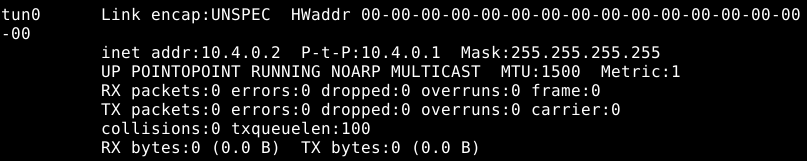
\includegraphics[width = \textwidth]{tun0}
        \caption{Características de tun0.}
      \end{figure}

      \par
      Los paquetes que vemos por eth1 no se pueden leer (figura
      \ref{figure:pingeth1}), en cambio por tun0 si podemos ver su contenido
      (figura \ref{figure:pingtun0}).

      \begin{figure}[H]
        \centering
        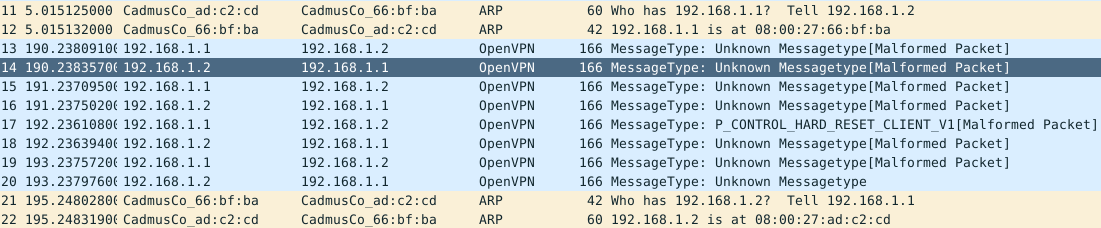
\includegraphics[width = \textwidth]{pingeth1}
        \caption{Paquetes por eth1.}
        \label{figure:pingeth1}
      \end{figure}

      \begin{figure}[H]
        \centering
        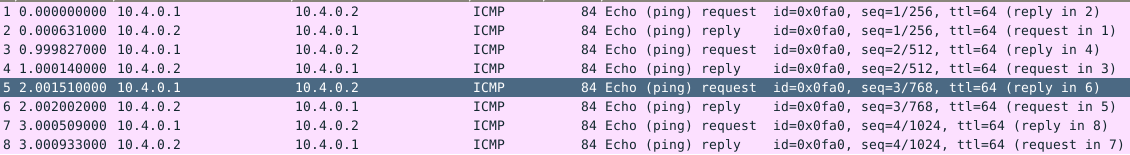
\includegraphics[width = \textwidth]{pingtun0}
        \caption{Paquetes por tun0.}
        \label{figure:pingtun0}
      \end{figure}

    \subsection{TLS con certificados}
    \par
    Salida del comando:\\
    sudo openvpn --remote 192.168.1.1 --dev tun --ifconfig 10.4.0.2 10.4.0.1 --tls-server --dh dh1024.pem --ca ca.crt --cert server.crt --key server.key --verb 4

\begin{lstlisting}
Sat Apr 21 20:07:46 2018 us=825293 Diffie-Hellman initialized with
1024 bit key
Sat Apr 21 20:07:46 2018 us=825524 WARNING: file 'server.key' is
group or others accessible
Sat Apr 21 20:07:46 2018 us=825784 Control Channel MTU parms
[ L:1541 D:138 EF:38 EB:0 ET:0 EL:0 ]
Sat Apr 21 20:07:46 2018 us=825848 Socket Buffers:
R=[229376->131072] S=[229376->131072]
Sat Apr 21 20:07:46 2018 us=826308 TUN/TAP device tun0 opened
Sat Apr 21 20:07:46 2018 us=826320 TUN/TAP TX queue length set
to 100
Sat Apr 21 20:07:46 2018 us=826328 do_ifconfig, tt->ipv6=0,
tt->did_ifconfig_ipv6_setup=0
Sat Apr 21 20:07:46 2018 us=826340 /sbin/ifconfig tun0
10.4.0.2 pointopoint 10.4.0.1 mtu 1500
Sat Apr 21 20:07:46 2018 us=827384 Data Channel MTU parms
[ L:1541 D:1450 EF:41 EB:4 ET:0 EL:0 ]
Sat Apr 21 20:07:46 2018 us=827400 Local Options String:
'V4,dev-type tun,link-mtu 1541,tun-mtu 1500,proto UDPv4,
ifconfig 10.4.0.1 10.4.0.2,cipher BF-CBC,auth SHA1,
keysize128,key-method 2,tls-server'
Sat Apr 21 20:07:46 2018 us=827404 Expected Remote Options
String: 'V4,dev-type tun,link-mtu 1541,tun-mtu 1500,
proto UDPv4,ifconfig 10.4.0.2 10.4.0.1,cipher BF-CBC,
auth SHA1,keysize 128,key-method 2,tls-client'
Sat Apr 21 20:07:46 2018 us=827415 Local Options hash
(VER=V4): 'bd0285da'
Sat Apr 21 20:07:46 2018 us=827420 Expected Remote Options
hash (VER=V4): '599bc3b6'
Sat Apr 21 20:07:46 2018 us=827425 UDPv4 link local (bound):
[undef]
Sat Apr 21 20:07:46 2018 us=827429 UDPv4 link remote:
[AF_INET]192.168.1.1:1194
Sat Apr 21 20:07:46 2018 us=827755 TLS: Initial packet from
[AF_INET]192.168.1.1:1194, sid=77b8cb72 79f522af
Sat Apr 21 20:07:46 2018 us=835973 VERIFY OK: depth=1,
/C=KG/ST=NA/L=BISHKEK/O=OpenVPN-TEST/emailAddress=me@myhost.mydomain
Sat Apr 21 20:07:46 2018 us=836137 VERIFY OK: depth=0,
/C=KG/ST=NA/O=OpenVPN-TEST/CN=Test-Client/emailAddress=me@myhost.mydomain
Sat Apr 21 20:07:46 2018 us=845402 Data Channel Encrypt:
Cipher 'BF-CBC' initialized with 128 bit key
Sat Apr 21 20:07:46 2018 us=845452 Data Channel Encrypt:
Using 160 bit message hash 'SHA1' for HMAC authentication
Sat Apr 21 20:07:46 2018 us=845501 Data Channel Decrypt:
Cipher 'BF-CBC' initialized with 128 bit key
Sat Apr 21 20:07:46 2018 us=845524 Data Channel Decrypt:
Using 160 bit message hash 'SHA1' for HMAC authentication
Sat Apr 21 20:07:46 2018 us=846128 Control Channel: TLSv1,
cipher TLSv1/SSLv3 DHE-RSA-AES256-SHA, 2048 bit RSA
Sat Apr 21 20:07:46 2018 us=846170 [Test-Client] Peer
Connection Initiated with [AF_INET]192.168.1.1:1194
Sat Apr 21 20:07:48 2018 us=70028 Initialization
Sequence Completed
\end{lstlisting}

      \bigskip
      \par
      Para configurar la VPN cliente-servidor hemos modificado el archivo left,
      configurandolo como cliente.
      \begin{lstlisting}
      client

      dev tun
      proto tcp
      remote 192.168.1.2 1194

      ca ca.crt
      cert client.crt
      key client.key

      remote-cert-tls server
      tls-remote Test-Server
      \end{lstlisting}

      \bigskip
      \par
      Y right lo hemos configurado como servidor.
      \begin{lstlisting}
      local 192.168.1.2
      port 1194
      proto tcp

      dev tun

      ca ca.crt
      cert server.crt
      key server.key

      dh dh2048.pem

      server 10.8.0.0 255.255.255.0

      ifconfig-pool-persist ipp.txt
      \end{lstlisting}


      \bigskip
      \par
      Una vez iniciada la VPN y aplicado el filtro en Wireshark vemos los
      siguientes mensajes, figura \ref{figure:tls}. En primer lugar el cliente
      saluda al servidor para inciar la conexión y este le contesta enviando
      sus datos de autenticación. Una vez autenticado el cliente envia sus datos
      y el servidor contesta enviando la información de la sesión.

      \begin{figure}[H]
        \centering
        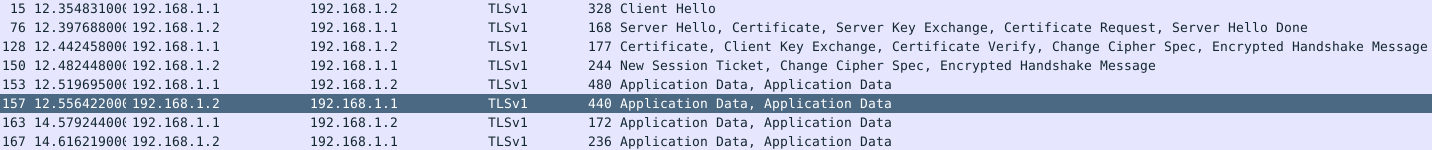
\includegraphics[width = \textwidth]{tls}
        \caption{Acuerdo TLS.}
        \label{figure:tls}
      \end{figure}


      \par
      Se puede escoger entre 45 conjuntos distintos, figura
      \ref{figure:ciphers}, de los cuales finalmente escogen solo uno que se
      puede ver en la figura \ref{figure:cipher}.

      \begin{figure}[H]
        \centering
        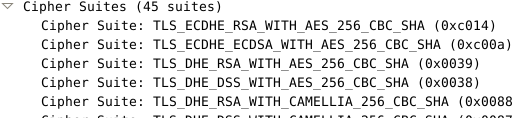
\includegraphics[width = \textwidth]{ciphers}
        \caption{Conjuntos de algoritmos.}
        \label{figure:ciphers}
      \end{figure}

      \begin{figure}[H]
        \centering
        
\includegraphics[width = \textwidth]{cipher}
        \caption{Conjunto escogido.}
        \label{figure:cipher}
      \end{figure}

      \par
      En certificate el cliente envia un certificado firmado que contiene su
      clave pública.


  \section{OpenSSH}
    \subsection{Autentificación con clave pública}
      \par
      La salida del comando ssh -v 192.168.1.2 es la siguiente.

\begin{lstlisting}
OpenSSH_6.0p1 Debian-4+deb7u7, OpenSSL 1.0.1e 11 Feb 2013
debug1: Reading configuration data /etc/ssh/ssh_config
debug1: /etc/ssh/ssh_config line 19: Applying options for *
debug1: Connecting to 192.168.1.2 [192.168.1.2] port 22.
debug1: Connection established.
debug1: identity file /home/usuario/.ssh/id_rsa type 1
debug1: Checking blacklist file /usr/share/ssh/blacklist.RSA-2048
debug1: Checking blacklist file /etc/ssh/blacklist.RSA-2048
debug1: identity file /home/usuario/.ssh/id_rsa-cert type -1
debug1: identity file /home/usuario/.ssh/id_dsa type -1
debug1: identity file /home/usuario/.ssh/id_dsa-cert type -1
debug1: identity file /home/usuario/.ssh/id_ecdsa type -1
debug1: identity file /home/usuario/.ssh/id_ecdsa-cert type -1
debug1: Remote protocol version 2.0, remote software version
  OpenSSH_6.0p1 Debian-4+deb7u7
debug1: match: OpenSSH_6.0p1 Debian-4+deb7u7 pat OpenSSH*
debug1: Enabling compatibility mode for protocol 2.0
debug1: Local version string SSH-2.0-OpenSSH_6.0p1 Debian-4+deb7u7
debug1: SSH2_MSG_KEXINIT sent
debug1: SSH2_MSG_KEXINIT received
debug1: kex: server->client aes128-ctr hmac-md5 none
debug1: kex: client->server aes128-ctr hmac-md5 none
debug1: sending SSH2_MSG_KEX_ECDH_INIT
debug1: expecting SSH2_MSG_KEX_ECDH_REPLY
debug1: Server host key: ECDSA c5:9d:97:b8:6e:87:e4:e3:cc:ec:3b:a8:bc:9e:8b:12
debug1: Host '192.168.1.2' is known and matches the ECDSA host key.
debug1: Found key in /home/usuario/.ssh/known_hosts:1
debug1: ssh_ecdsa_verify: signature correct
debug1: SSH2_MSG_NEWKEYS sent
debug1: expecting SSH2_MSG_NEWKEYS
debug1: SSH2_MSG_NEWKEYS received
debug1: SSH2_MSG_SERVICE_REQUEST sent
debug1: SSH2_MSG_SERVICE_ACCEPT received
debug1: Authentications that can continue: publickey,password
debug1: Next authentication method: publickey
debug1: Offering RSA public key: /home/usuario/.ssh/id_rsa
debug1: Server accepts key: pkalg ssh-rsa blen 279
debug1: key_parse_private_pem: PEM_read_PrivateKey failed
debug1: read PEM private key done: type <unknown>
Enter passphrase for key '/home/usuario/.ssh/id_rsa':
debug1: read PEM private key done: type RSA
debug1: Authentication succeeded (publickey).
Authenticated to 192.168.1.2 ([192.168.1.2]:22).
debug1: channel 0: new [client-session]
debug1: Requesting no-more-sessions@openssh.com
debug1: Entering interactive session.
debug1: Sending environment.
debug1: Sending env LANG = es_ES.UTF-8
Linux debian 3.2.0-4-amd64 #1 SMP Debian 3.2.63-2 x86_64

The programs included with the Debian GNU/Linux system are free software;
the exact distribution terms for each program are described in the
individual files in /usr/share/doc/*/copyright.

Debian GNU/Linux comes with ABSOLUTELY NO WARRANTY, to the extent
permitted by applicable law.
Last login: Sat Apr 21 19:29:26 2018
\end{lstlisting}

    \subsection{Reenvío de puertos}
      \par
      \textbf{ssh -v -N -L 8080:www.ucm.es:80 usuario@192.168.1.2}

\begin{lstlisting}
OpenSSH_6.0p1 Debian-4+deb7u7, OpenSSL 1.0.1e 11 Feb 2013
debug1: Reading configuration data /etc/ssh/ssh_config
debug1: /etc/ssh/ssh_config line 19: Applying options for *
debug1: Connecting to 192.168.1.2 [192.168.1.2] port 22.
debug1: Connection established.
debug1: identity file /home/usuario/.ssh/id_rsa type -1
debug1: identity file /home/usuario/.ssh/id_rsa-cert type -1
debug1: identity file /home/usuario/.ssh/id_dsa type -1
debug1: identity file /home/usuario/.ssh/id_dsa-cert type -1
debug1: identity file /home/usuario/.ssh/id_ecdsa type -1
debug1: identity file /home/usuario/.ssh/id_ecdsa-cert type -1
debug1: Remote protocol version 2.0, remote software version OpenSSH_6.0p1 Debian-4+deb7u7
debug1: match: OpenSSH_6.0p1 Debian-4+deb7u7 pat OpenSSH*
debug1: Enabling compatibility mode for protocol 2.0
debug1: Local version string SSH-2.0-OpenSSH_6.0p1 Debian-4+deb7u7
debug1: SSH2_MSG_KEXINIT sent
debug1: SSH2_MSG_KEXINIT received
debug1: kex: server->client aes128-ctr hmac-md5 none
debug1: kex: client->server aes128-ctr hmac-md5 none
debug1: sending SSH2_MSG_KEX_ECDH_INIT
debug1: expecting SSH2_MSG_KEX_ECDH_REPLY
debug1: Server host key: ECDSA c5:9d:97:b8:6e:87:e4:e3:cc:ec:3b:a8:bc:9e:8b:12
The authenticity of host '192.168.1.2 (192.168.1.2)' can't be established.
ECDSA key fingerprint is c5:9d:97:b8:6e:87:e4:e3:cc:ec:3b:a8:bc:9e:8b:12.
Are you sure you want to continue connecting (yes/no)? yes
Warning: Permanently added '192.168.1.2' (ECDSA) to the list of known hosts.
debug1: ssh_ecdsa_verify: signature correct
debug1: SSH2_MSG_NEWKEYS sent
debug1: expecting SSH2_MSG_NEWKEYS
debug1: SSH2_MSG_NEWKEYS received
debug1: SSH2_MSG_SERVICE_REQUEST sent
debug1: SSH2_MSG_SERVICE_ACCEPT received
debug1: Authentications that can continue: publickey,password
debug1: Next authentication method: publickey
debug1: Trying private key: /home/usuario/.ssh/id_rsa
debug1: Trying private key: /home/usuario/.ssh/id_dsa
debug1: Trying private key: /home/usuario/.ssh/id_ecdsa
debug1: Next authentication method: password
usuario@192.168.1.2's password:
debug1: Authentication succeeded (password).
Authenticated to 192.168.1.2 ([192.168.1.2]:22).
debug1: Local connections to LOCALHOST:8080 forwarded to remote address www.ucm.es:80
debug1: Local forwarding listening on ::1 port 8080.
debug1: channel 0: new [port listener]
debug1: Local forwarding listening on 127.0.0.1 port 8080.
debug1: channel 1: new [port listener]
debug1: Requesting no-more-sessions@openssh.com
debug1: Entering interactive session.
\end{lstlisting}

      \bigskip
      \par
      \textbf{ssh -v -X -R 8080:www.ucm.es:80 usuario@192.168.1.2 chromium}\\
      Da un fallo al abrir chromium por lo que no hemos podido verlo pero
      suponemos que la interfaz se abrira en lef, la que ejecuta el comando. El
      puerto 8080 que esta escuchando es el de right.

\begin{lstlisting}
debug1: Authentication succeeded (password).
Authenticated to 192.168.1.2 ([192.168.1.2]:22).
debug1: Remote connections from LOCALHOST:8080 forwarded to local address
  www.ucm.es:80
debug1: channel 0: new [client-session]
debug1: Requesting no-more-sessions@openssh.com
debug1: Entering interactive session.
debug1: remote forward success for: listen 8080, connect www.ucm.es:80
debug1: All remote forwarding requests processed
debug1: Sending environment.
debug1: Sending env LANG = es_ES.UTF-8
debug1: Sending command: chromium
[3460:3460:0421/213125:ERROR:browser_main_loop.cc(207)] Gtk: cannot open
  display:
debug1: client_input_channel_req: channel 0 rtype exit-status reply 0
debug1: client_input_channel_req: channel 0 rtype eow@openssh.com reply 0
debug1: channel 0: free: client-session, nchannels 1
Transferred: sent 1880, received 1728 bytes, in 0.0 seconds
Bytes per second: sent 48793.0, received 44848.0
debug1: Exit status 1
\end{lstlisting}

      \bigskip
      \par
      \textbf{ssh -v -N -D 1080 usuario@192.168.1.2}\\
      Para el servidor la maquina que quiere conectarse es right, que es la que
      hace de proxy.

\begin{lstlisting}
debug1: Authentication succeeded (password).
Authenticated to 192.168.1.2 ([192.168.1.2]:22).
debug1: Local connections to LOCALHOST:1080 forwarded to remote address
  socks:0
debug1: Local forwarding listening on ::1 port 1080.
debug1: channel 0: new [port listener]
debug1: Local forwarding listening on 127.0.0.1 port 1080.
debug1: channel 1: new [port listener]
debug1: Requesting no-more-sessions@openssh.com
debug1: Entering interactive session.
\end{lstlisting}

\end{document}
